The first step of the HLT processing is to run on the RoIs found by the L1 hardware trigger. These
RoIs are collected and distributed to the HLT farm by the RoIB \cite{1748-0221-11-02-C02080} which was the 
latest change to the ATLAS dataflow. 
%This system was installed in ATLAS
% between the 2015 and 2016 data taking periods. 
The
evolution of the RoIB system from a crate of custom VME-based electronics (VME-RoIB) to a commodity
PC hosting a custom PCI-Express card (PC-RoIB) has been undertaken to increase the system performance,
flexibility, and ease of maintenance. The functionality of the VME-RoIB previously possible only in FPGAs has
now been implemented in a multi-threaded C++ software library. 
For each proton-proton collision that is accepted by the L1 trigger, the
RoIB receives an RoI record from the custom inputs via S-Link. The RoIB assembles these records into
a single record which is then forwarded to the HLTSV. The HLTSV then
distributes these single records to the HLT farm. The RoIB is also responsible for monitoring the
data integrity of the incoming fragments and diagnostic performance of the system.

As shown in Figure \ref{fig:roib_summary}, the performance of the PC-RoIB with realistic running ATLAS conditions
is improved over the VME-RoIB particularly at high RoI sizes. 

\begin{figure}[t!]
\centering
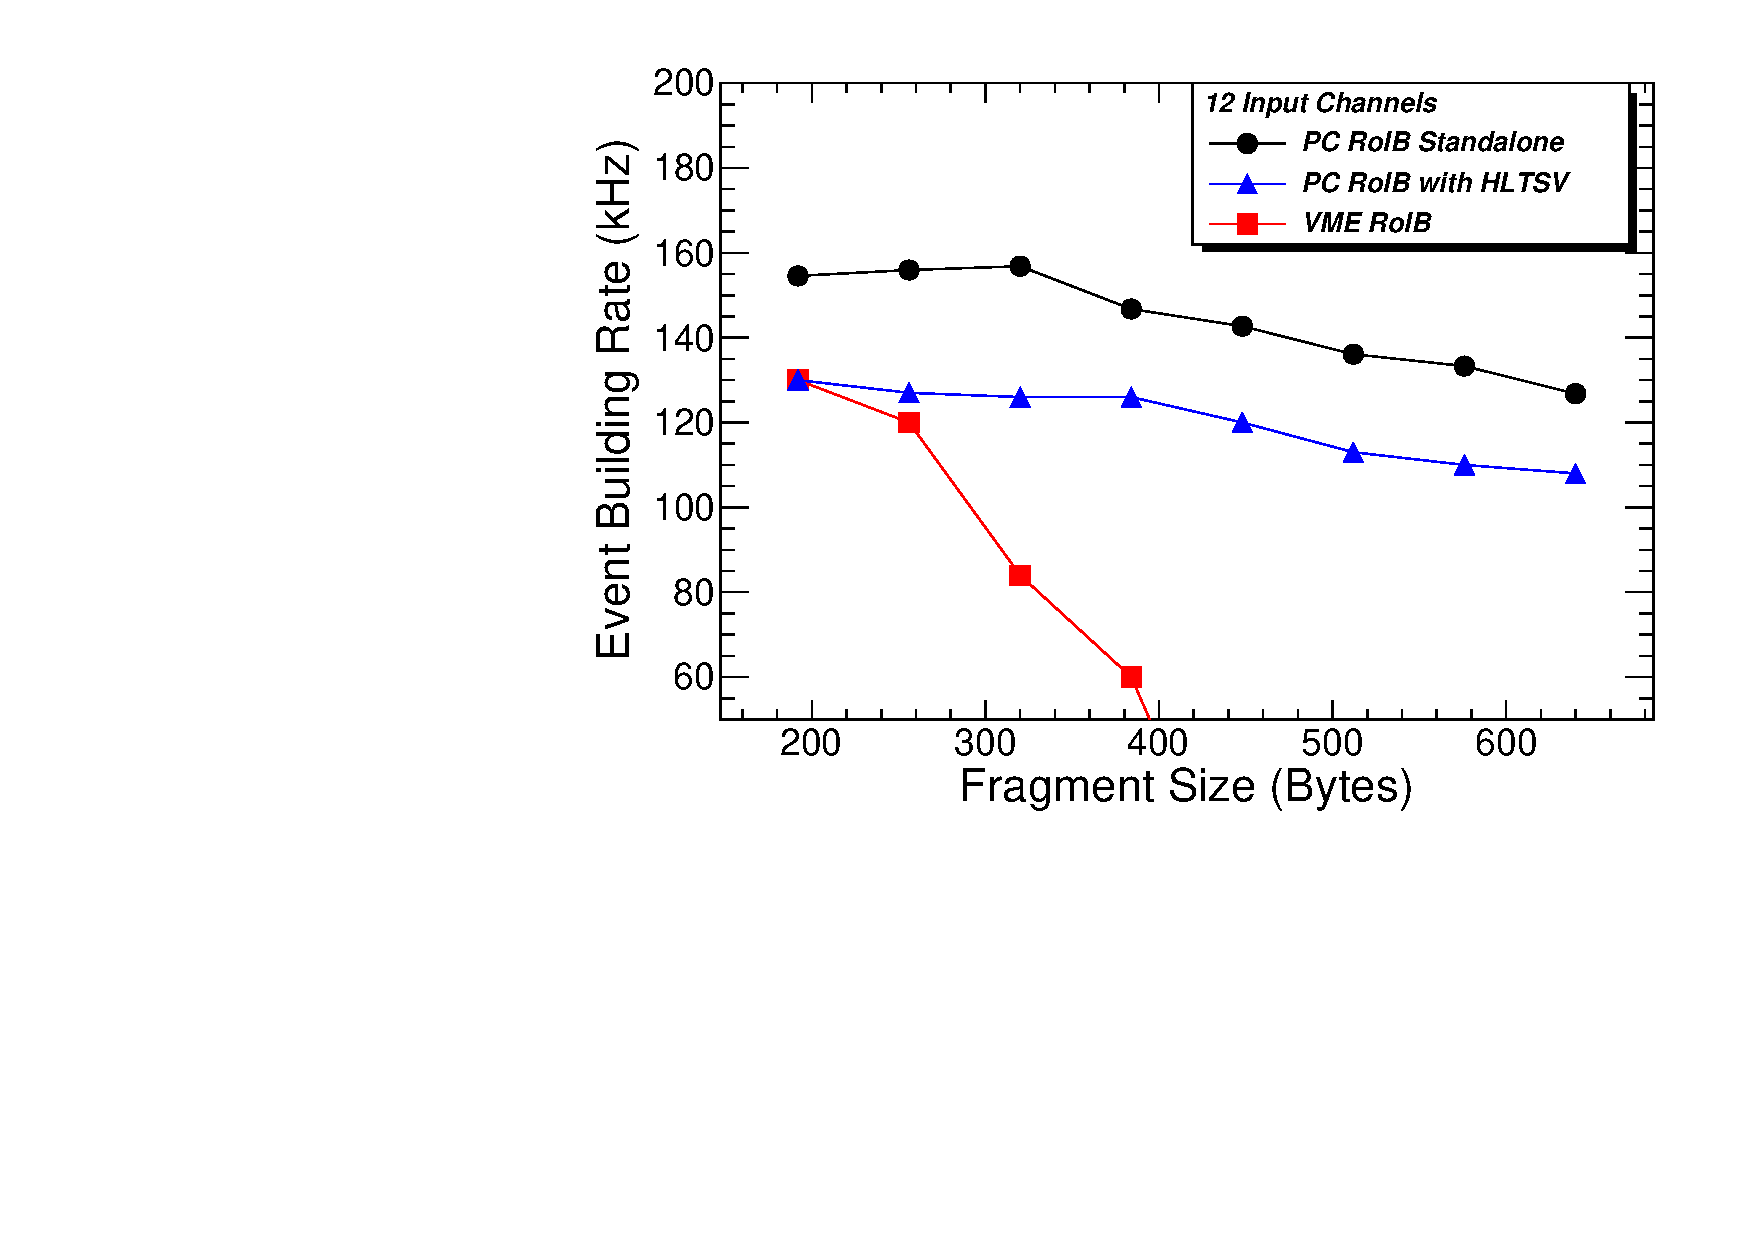
\includegraphics[width=0.5\textwidth]{roib_summary_size} 
\caption{The event building rate as a function of the RoI record size in Bytes. The rates are shown for a standalone application that implements 
a minimal interface for event building, the integrated RoIB software into an HLTSV process
running within the full ATLAS TDAQ software suite, and for comparison the VME-RoIB performance.}
\label{fig:roib_summary}
\end{figure} 

Figure \ref{fig:roib_pileup_l1rate} shows that the memory usage of the HLTSV is at the level of 5\% and that the RoIB event assembly does not depend 
on pileup conditions.


\begin{figure}[t!]
\centering
\begin{subfigure}[t]{0.48\textwidth}
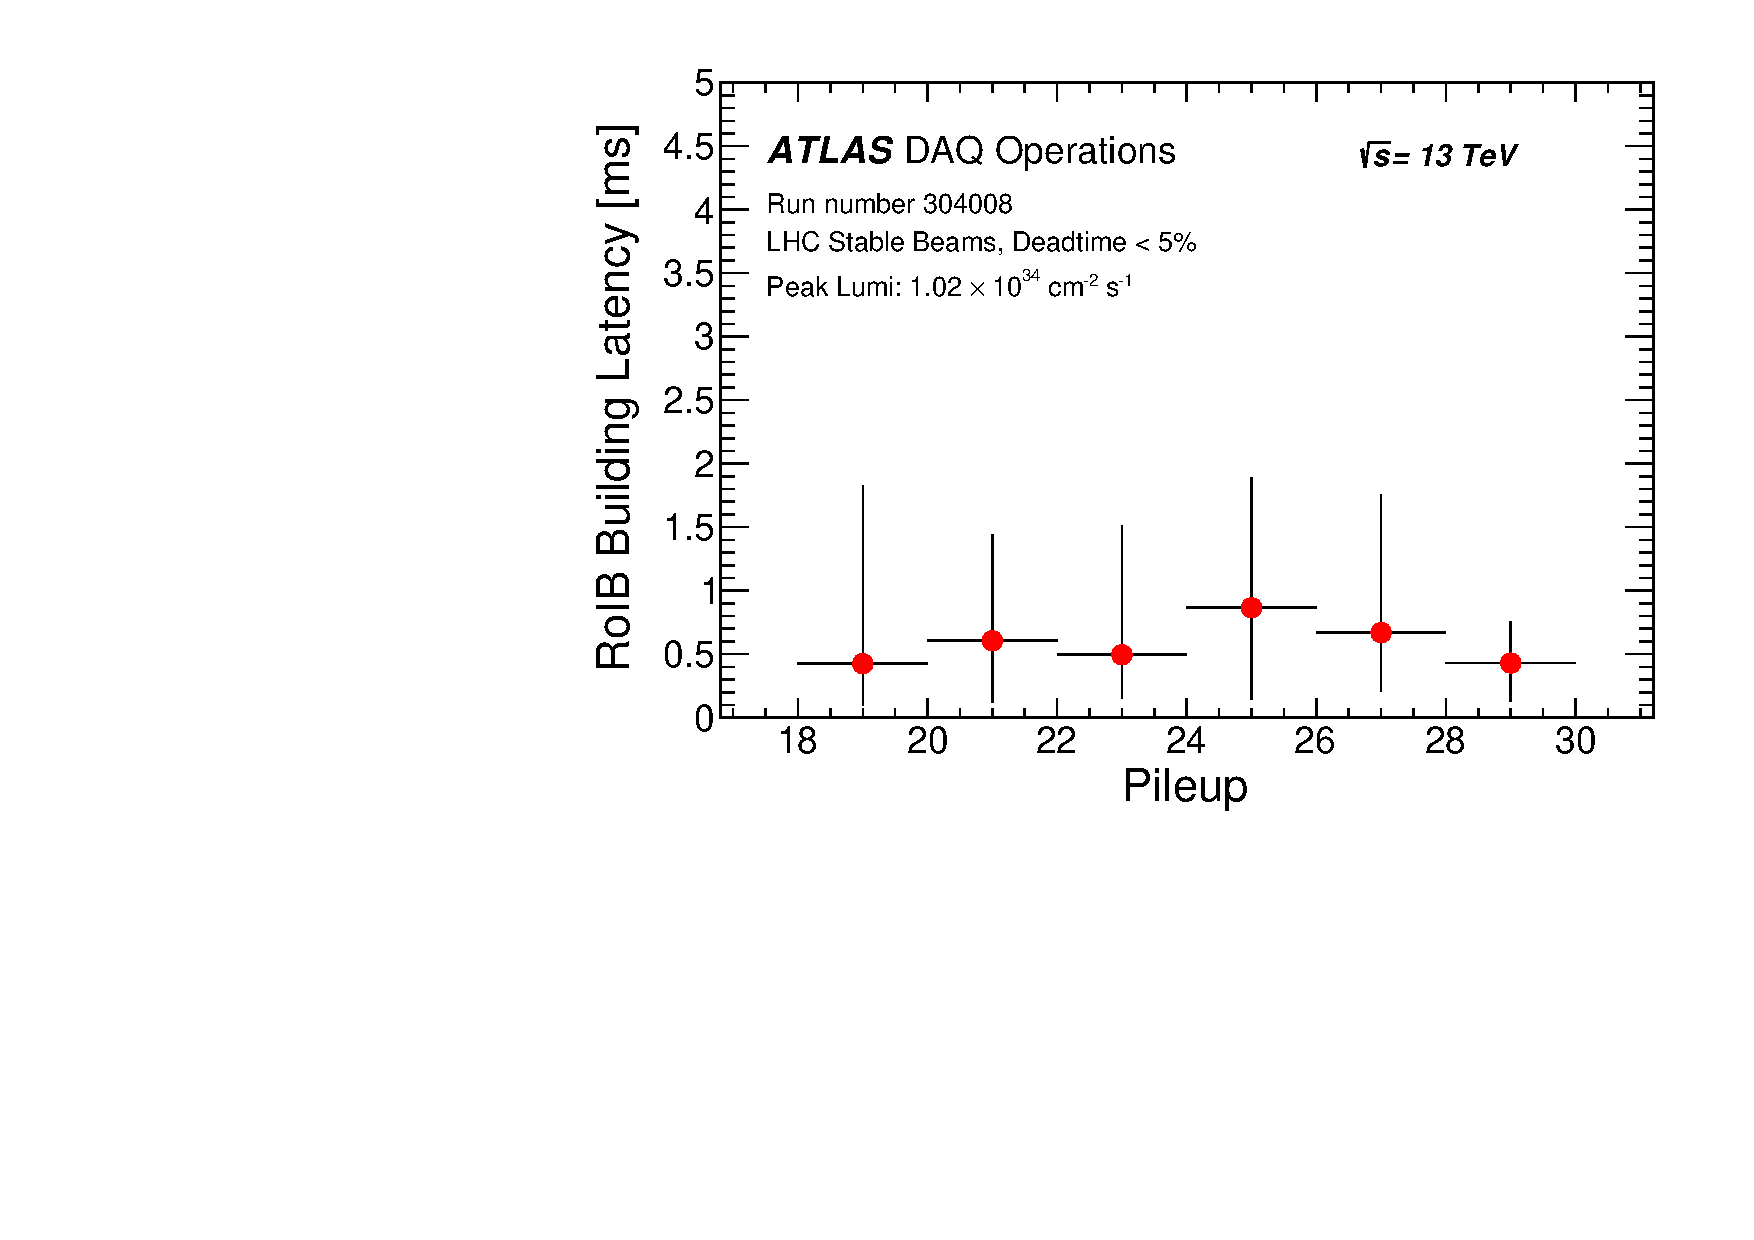
\includegraphics[width=0.95\textwidth]{GrAssym_run_304008_pileup_RoIBbuildtime}
\end{subfigure}
\begin{subfigure}[t]{0.48\textwidth}
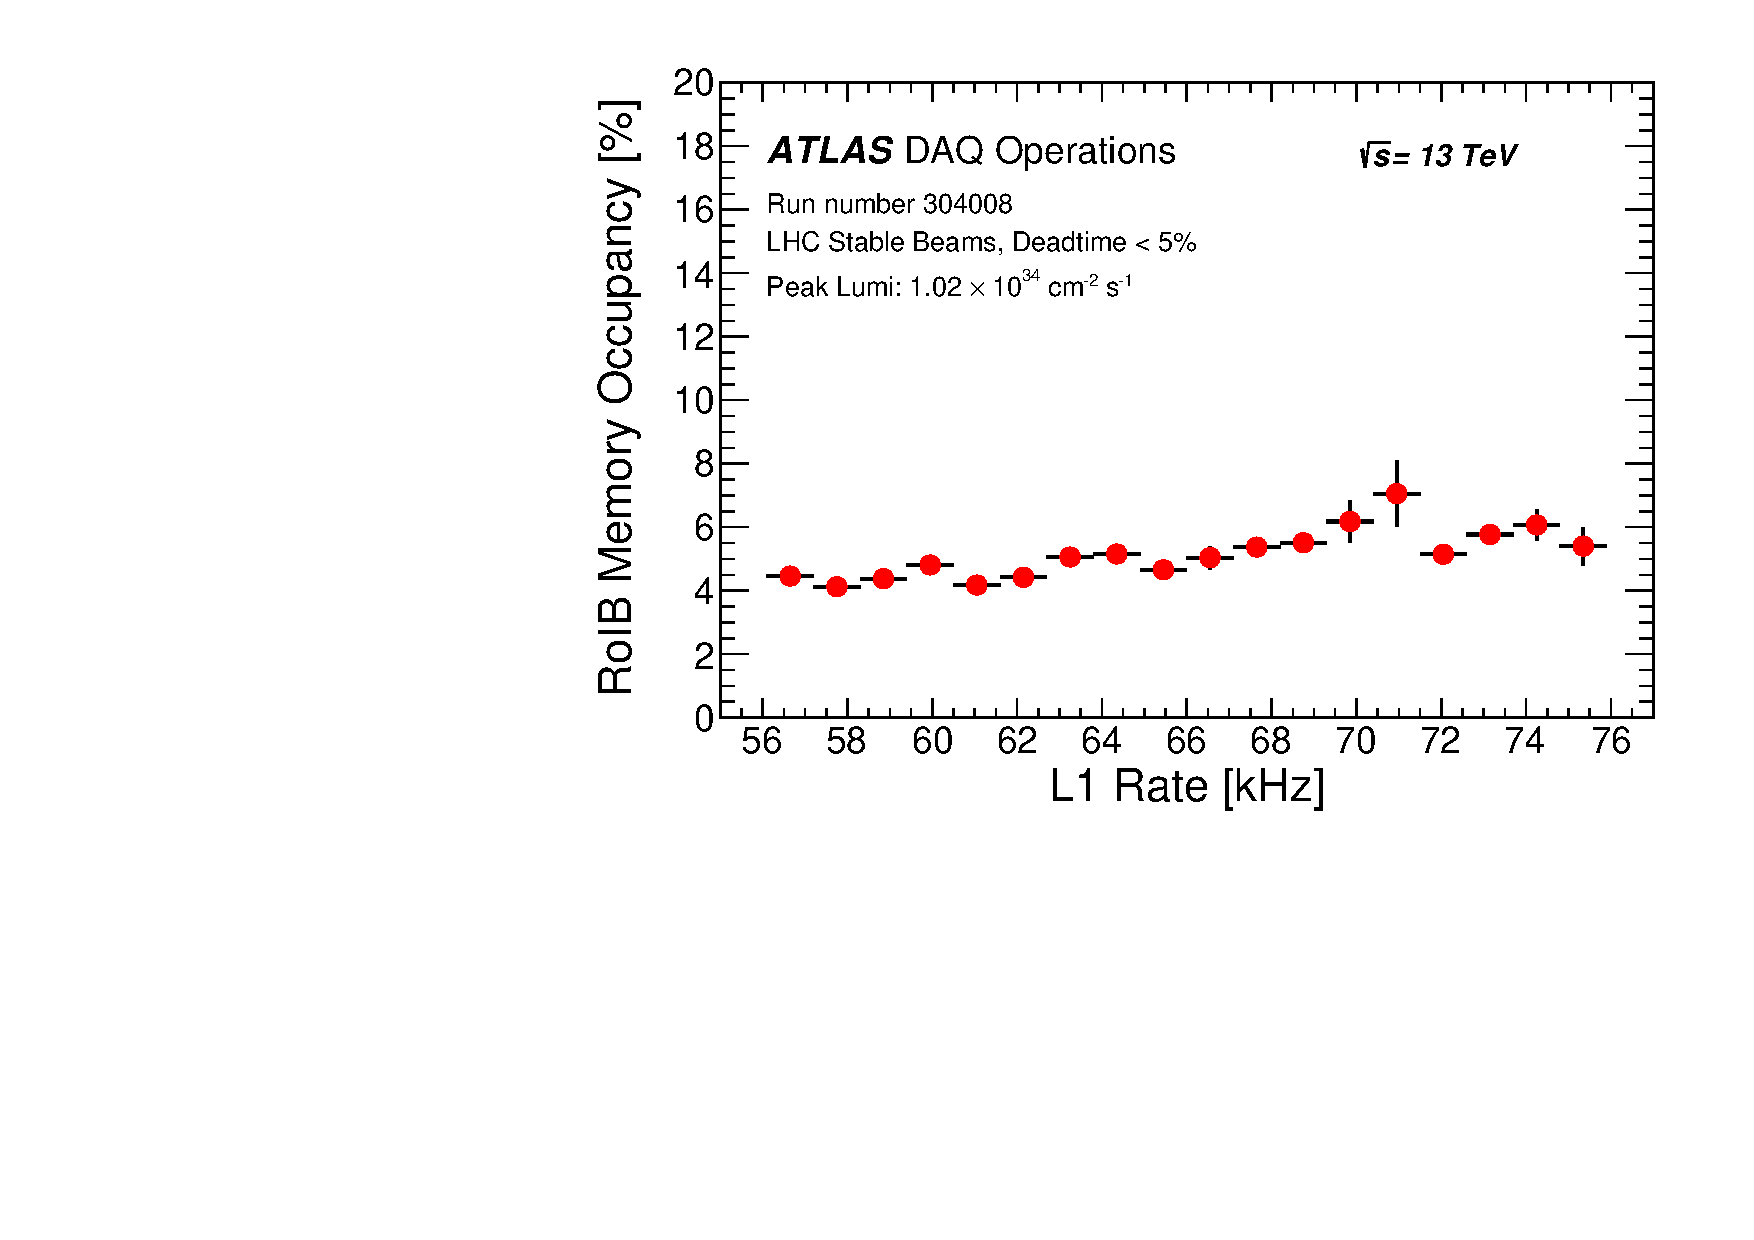
\includegraphics[width=0.95\textwidth]{hProf_run_304008_l1rate_RoIBMemOccup}
\end{subfigure}
\vspace{-0.25cm}
\caption{RoIB performance: RoIB building latency as a function of pileup (left), RoIB memory occupancy as a function of L1 rate (right).}
\label{fig:roib_pileup_l1rate}
\end{figure} 


